\documentclass[12pt]{article}
\usepackage[usenames]{color}
\usepackage{graphicx}
\usepackage{verbatim}



% begin preamble
\setlength{\baselineskip}{16.0pt}    % 16 pt usual spacing between lines

\setlength{\parskip}{3pt plus 2pt}
\setlength{\parindent}{20pt}
\setlength{\oddsidemargin}{0.5cm}
\setlength{\evensidemargin}{0.5cm}
\setlength{\marginparsep}{0.75cm}
\setlength{\marginparwidth}{2.5cm}
\setlength{\marginparpush}{1.0cm}
\setlength{\textwidth}{150mm}

\pagestyle{empty} % use if page numbers not wanted

% end preamble

\begin{document}
\title{Amanzi Build System Design}

\section{Use Cases}
\subsection{End-User}
This user is familiar with running simple scripts, RPM commands, Windows Install Wizard or Mac DMG files,
however Amanzi is a black-box solver and the user has little or no knowledge of the complete architecture
of the software.
Number of steps to build Amanzi from a distribution tar file in this case should be no more than untar the file,
select build options (structured vs. unstructured, installation location, etc.) and run make.  The 
build system must make intelligent choices such searching for required TPLs and building these
TPLs if they are not located or the version found is not a valid configuration for Amanzi.

\subsection{Developer/Advanced User}
This user is much more familiar with the overall design of Amanzi and will require a custom configuration
of both Amanzi and TPLs. This user may mix Amanzi built TPLs and custom built TPLs. \textcolor{red}{In this use case, it
is required that any specified TPL be used over any build system built TPL or found system TPL.} 

\subsection{Distribution}
The Amanzi environment must have a well-defined reproducible way to create and distribute source code, libraries
and binaries. When distributing libraries and binaries, they must be built with consistent TPLs. This requires the build
system to generate source code tar files and binary distributions that may (or will eventually) include RPM files,
DMG files and pre-built binaries and libraries. \textcolor{red}{The V\&V usage model falls under this use case and it
is critical that how the Amanzi is built is documented with controls on what is enabled and built.}

\section{Requirements}
\begin{itemize}
\item The build system will build and install required TPLs if the user has not specified the location of the TPL or
          the build system can not locate an acceptable version of the TPL.
\item When the user does specify a particular TPL installation to use, this choice will always supersede any other
          TPL definitions or configuration in the build system.
\item The default behavior for the build system shall be
\begin{itemize}
\item Search the system for the TPL. The search path criteria will be:
\begin{itemize}
\item User specified XXX\_DIR location,
\item CMake default search paths
\end{itemize}
\item If the search fails or the TPL found does not meet Amanzi software requirements, then the TPL will be built
          along with the Amanzi software.          
\end{itemize}
\item The build system shall define the contents of a source code distribution tar file and create this tar file.
\item The build system shall define a binary distribution of the Amanzi libraries and binaries configured for various
          OS platforms.
\item No matter what method the build system selects to import a TPL into the Amanzi build system, the build system 
          will define the following variables for each TPL:
\begin{itemize}
\item XXX\_FOUND = Boolean flag indicating if the TPL has been found
\item BUILD\_XXX = Boolean flag indicating if the TPL will be built as an External project.
\item XXX\_INCLUDE\_DIR = Directory containing the TPL include files.
\item XXX\_INCLUDE\_DIRS = List of directories containing ALL required include files.
\item XXX\_LIBRARY\_DIR = Location of the TPL library installation path
\item XXX\_LIBRARIES = List of library directories required to link against the TPL
\end{itemize}
\item For each required and optional TPL, the build system shall have one location where the source, configuration,
          minimum version requirements, patching steps, and default download, build and install locations are defined.
\item When the build system is required or asked to build a TPL, the user will have the option to control the download,
          build and installation locations.
\item The user shall not have control over the minimum version requirements or TPL configuration in the build system.
\item  The build system will have a bootstrap capability that will search for CMake, verify the version available and test 
           that CMake is configured to handle the test dashboard capability.                   
                            
\end{itemize}

\section{Design}

\subsection{ExternalProject\_Add}
With version release 2.8, CMake now provides a module called ExternalProject that allows projects to configure, build
and install external software dependencies. We will use this functionality to create TPL installations that meet Amanzi
software requirements. The module can access the source from repositories, download archive files or access local copies 
of archive files, build, install and test source with standard build tools such as CMake and GNU Autotools. 
\textcolor{red}{Current build system requires version 2.8.2 or later. Depending on ExternalProject will not change the
Cmake version requirements.}

\subsection{Code Organization}
In the build branch of the Amanzi source repository, we will create a new directory {SuperBuild} at the root source level.
In this directory we will define a new project called {AmanziSuperBuild}. Under this project,  the configuration definition
and build controls for each TPL target will reside. The CMakeList.txt file in this directory will define general configuration
flags, such as shared library builds, compilers, compiler flags and build types. It will also have the logic that controls
when a TPL is built and include the build CMake file.

\subsection{TPLVersions.cmake}
This file will define the version, source file access location, and in the case of archive files, the archive file name and MD5
sum value for verification purposes. The variable definitions for each TPL will be,
\begin{itemize}
\item XXX\_VERSION\_MAJOR: Major version number
\item XXX\_VERSION\_MINOR: Minor version number
\item XXX\_VERSION\_PATCH: Patch version number
\item XXX\_VERSION\_STRING: String that identifies the version
\item XXX\_ARCHIVE\_FILE: tar, zip file containing the source
\item XXX\_MD5\_SUM: MD5 sum of archive file
\end{itemize}

\subsection{BuildXXX.cmake}
For each TPL there will be a file called BuildXXX.cmake that will define all the configuration, build and install
requirements. This file will be included in the CMakeList.txt file.

By default, each TPL will be un-tar'd, built and installed in a directory  in the root CMAKE\_BINARY\_DIR directory
called external-projects and then under a subdirectory with the TPL name.


\subsection{Sample BuildCURL.cmake}
\begin{verbatim}

#
# This include defines
# CURL_VERSION_STRING=7.21.6
# CURL_DOWNLOAD_LOCATION=<some local directory>
# CURL_ARCHIVE_FILE=curl-${CURL_VERSION_STRING}.tar.gz
# CURL_MD5_SUM=
include(TPLVersions)

# Define source, build and install directories
set(CURL_source_dir "${CMAKE_BINARY_DIR}/external-projects/curl")
set(CURL_binary_dir "${CMAKE_BINARY_DIR}/external-projects/curl-build")
set(CURL_install_dir "${CMAKE_BINARY_DIR}/external-projects/curl")

# Make target: build curl with 'make curl' command
set(CURL_target curl)

# Add the external project and tie to curl target
ExternalProject_Add(
    ${CURL_target}
    SOURCE_DIR ${CURL_source_dir}
    BINARY_DIR ${CURL_binary_dir}
    INSTALL_DIR ${CURL_install_dir}
    URL ${CURL_DOWNLOAD_LOCATION}/${CURL_ARCHIVE_FILE}
    URL_MD5 ${CURL_MD5_SUM}
    CONFIGURE_COMMAND
                   <SOURCE_DIR>/configure
                                                --prefix=<INSTALL_DIR>
                                                 ${AMANZI_COMMON_CONFIG_OPTIONS}
)
                                      
# Define variables needed by other packages
set(CURL_INCLUDE_DIR "${CURL_install_dir}/include")
set(CURL_INCLUDE_DIRS "${CURL_install_dir}/include")

# We'll need a macro to build library name when shared is on or off
define_library_name(curl BUILD_SHARED CURL_LIBRARY)
set(CURL_LIBRARIES "${CURL_LIBRARY}")

                                       
\end{verbatim}

\subsection{Flow Charts}

\begin{figure}
\begin{center}
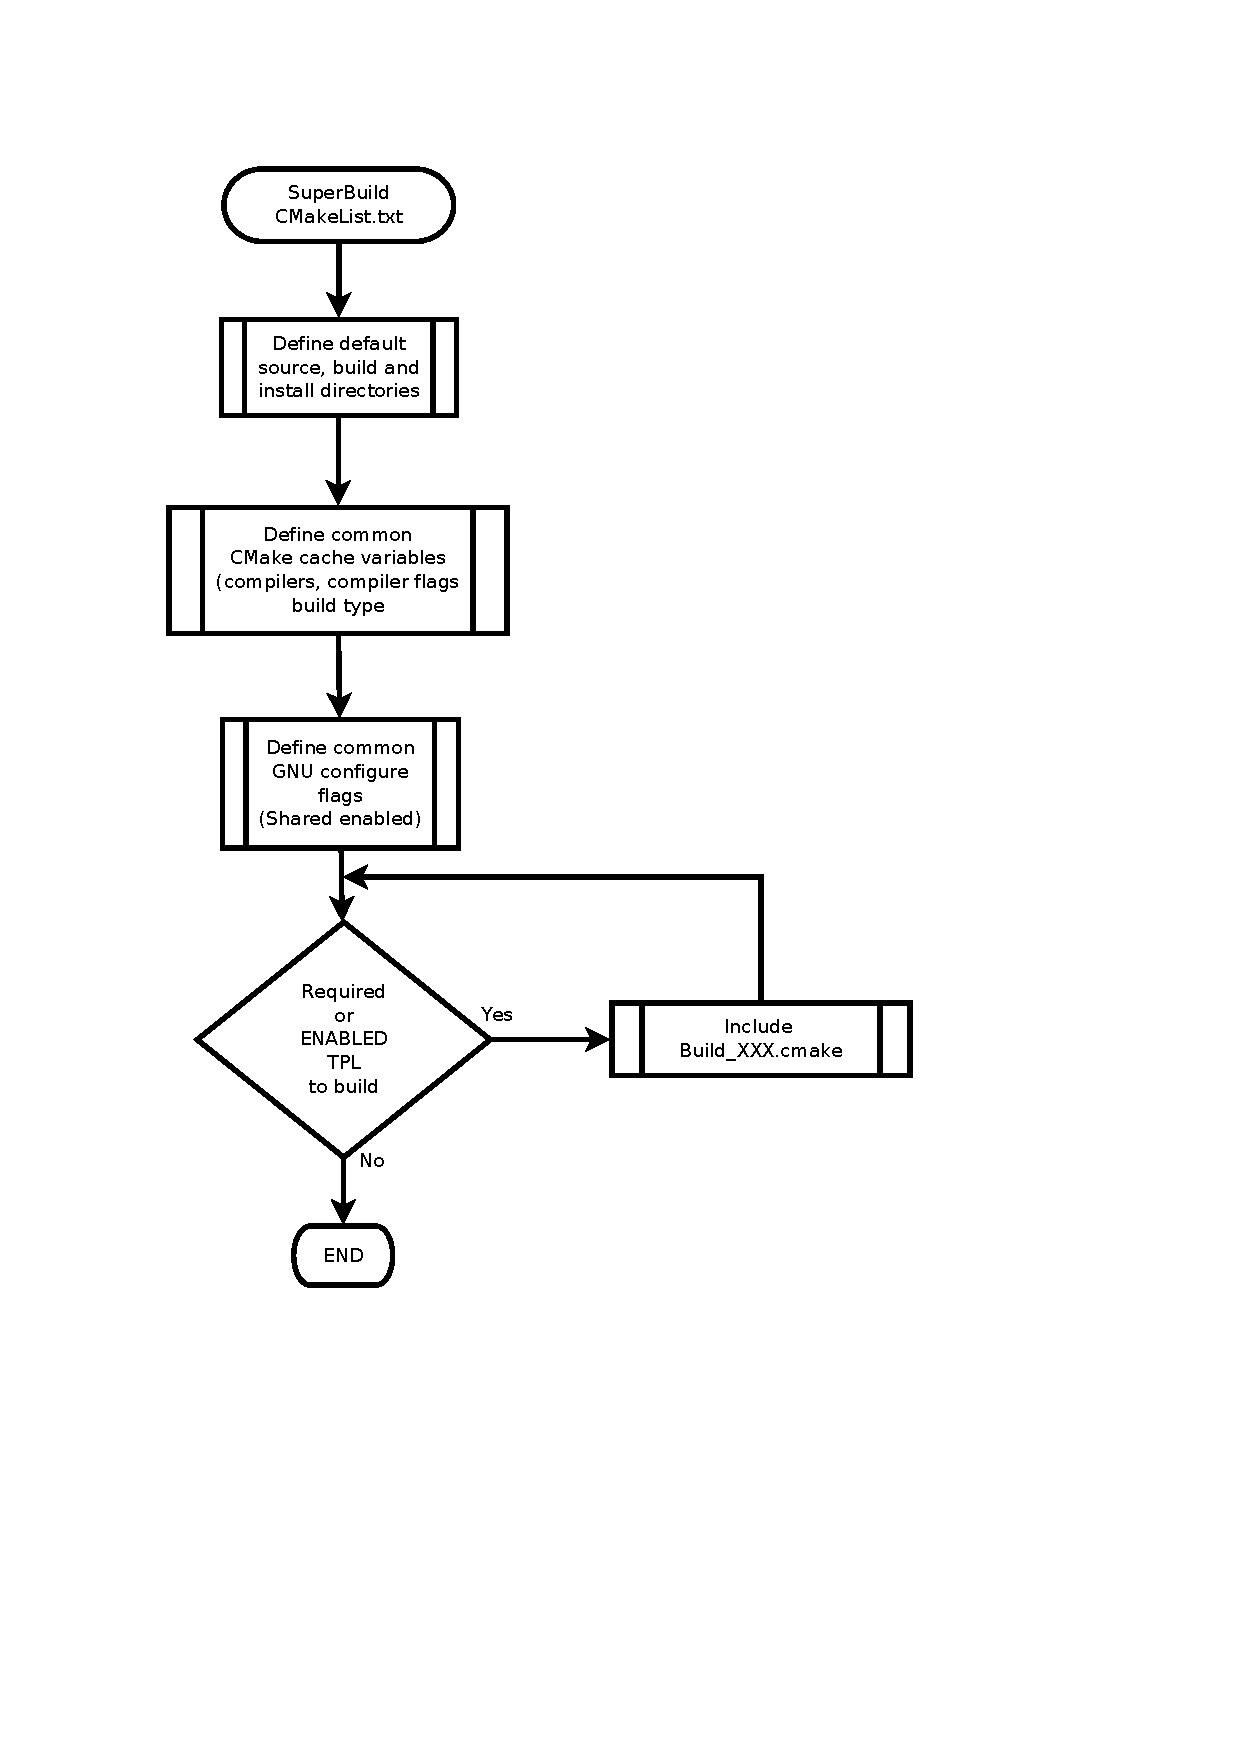
\includegraphics[width=1.0\textwidth]{figures/SuperBuildCMakeList.pdf}
\end{center}
\caption{SuperBuild CMakeList.txt flow logic}
\end{figure}


\begin{figure}
\begin{center}
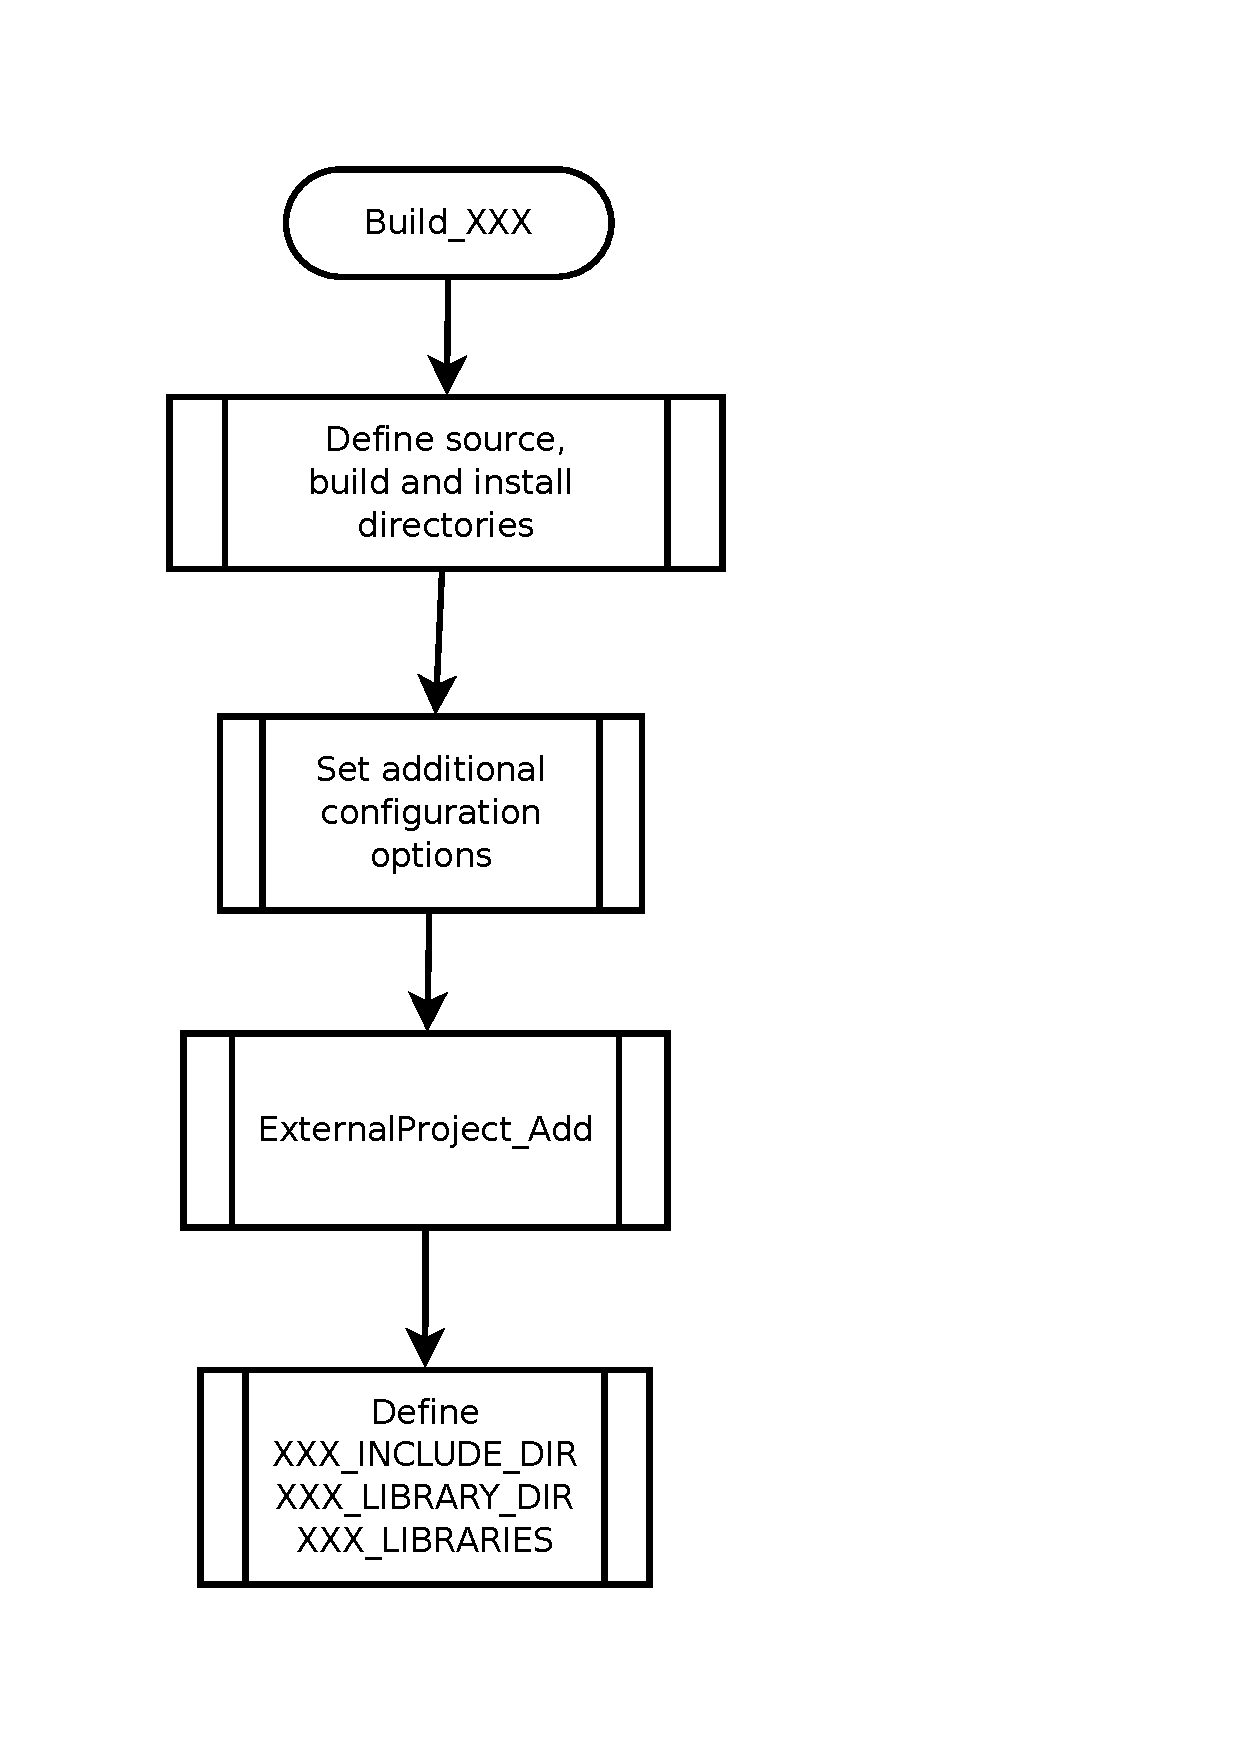
\includegraphics[scale=0.5]{figures/Build_XXX.pdf}
\end{center}
\caption{Generic Build\_XXX.cmake flow logic}
\end{figure}




 
   
\end{document}
